\documentclass[xcolor=dvipsnames]{beamer}

\setbeamertemplate{navigation symbols}{}
% \setbeamertemplate{background}[grid][step=1cm]
\useoutertheme{infolines}
\usecolortheme[named=violet]{structure}
\setbeamertemplate{items}[circle]

\usepackage{tikz}
\usetikzlibrary{arrows,shapes,backgrounds}
\usepackage{listings}
\usepackage{graphicx}
\usepackage{color}
\usepackage{hyperref}
\usepackage{xspace}

\usepackage{courier}


\hypersetup{colorlinks=true}

\newcommand{\app}[1]{\textbf{\textit{#1}}\xspace}
\def\waf{\app{waf}}
\def\hwaf{\app{hwaf}}
\def\worch{\app{worch}}

\newcommand{\git}{\texttt{\textbf{git}}\xspace}
\author[Brett Viren]{Brett Viren}
\title[ILCRoot]{Status of ORKA' ILCRoot \\ Repository Migration and Installation}
\date{ORKA Sim 2013/10/07}


\begin{document}

\lstset{%
  emphstyle=\color{red},
  keywordstyle=\color{black}\bfseries,
  basicstyle=\footnotesize\ttfamily,
  identifierstyle=\color{DarkOrchid}\ttfamily,
  commentstyle=\color{Brown}\ttfamily,
  stringstyle=\color{blue}\ttfamily,
  showstringspaces=false}


\begin{frame}
  \titlepage
\end{frame}

\section{Repository}

\begin{frame}
  \frametitle{Repository (Re)Migration}

  \begin{itemize}
  \item This time taken from SVN at\\
    \url{http://m65g.fnal.gov:9880/ilcroot_orka}
    \begin{itemize}
    \item[$\rightarrow$] We should now turn off commits.
    \item[$\rightarrow$] Developers should move to the new Redmine/\git (see next)
    \end{itemize}
  \item Migration points:
    \begin{itemize}
    \item Last one: r50 / 2012-12-03
    \item This one: r191 / 2013-09-24
    \end{itemize}
  \item The past few build related fixes have been re-based and committed.
  \item Initial build tests okay but more in-depth testing and use is needed.
  \end{itemize}

  A re-re-migration is not expected.  \\
  If any \git-related problems
  happen to pop up, let's just fix them.

\end{frame}

\begin{frame}
  \frametitle{ORKA ILCRoot Redmine}
  Redmine project at:
  \begin{center}
    \url{https://cdcvs.fnal.gov/redmine/projects/orka-ilcroot}
  \end{center}
  Requires FNAL ``services'' and/or Kerberos accounts for some access.
  \begin{description}
  \item[\href{https://cdcvs.fnal.gov/redmine/projects/orka-ilcroot/wiki}{wiki}]
    \begin{itemize}
    \item world readable
    \item requires Redmine ``Developer'' role to edit.
    \item holds (old) installation and general \git instructions
    \end{itemize}
  \item[\href{https://cdcvs.fnal.gov/redmine/projects/orka-ilcroot/repository}{repo}] 
    \begin{itemize}
    \item \href{http://cdcvs.fnal.gov/projects/orka-ilcroot}{world read-only} 
      and 
      \href{ssh://p-orka-ilcroot@cdcvs.fnal.gov/cvs/projects/orka-ilcroot}{authenticated commits}
      to \git
    \item commits need Redmine ``Developer'' role and Kerberos
    \item multiple \git{}s possible: suggest secondary repo(s) to hold
      personal ILCRoot analysis code
    \end{itemize}
  \item[\href{https://cdcvs.fnal.gov/redmine/projects/orka-ilcroot/issues}{issues}]
    \begin{itemize}
    \item for bug reports, feature requests, expected milestones
    \item requires Redmine ``Reporter'' role to add issues
    \item so far unused, but can be very useful
    \end{itemize}
  \end{description}

  
\end{frame}

\section{Installation}

\begin{frame}[fragile]
  \frametitle{ILCRoot + Externals}
  \vspace{-7mm}

  \begin{columns}
    \begin{column}{0.5\textwidth}
      \begin{enumerate}
      \item       cmake
      \item     gccxml
      \item    geant
      \item     geant3vmc
      \item geant4vmc
      \item ilcroot
      \item   pythia
      \item    python
      \item    root
      \item      vgm
      \item       xerces-c
      \end{enumerate}
      {\footnotesize Relatively small project.
        Figure shows build steps and their dependencies.}
    \end{column}
    \begin{column}{0.5\textwidth}
      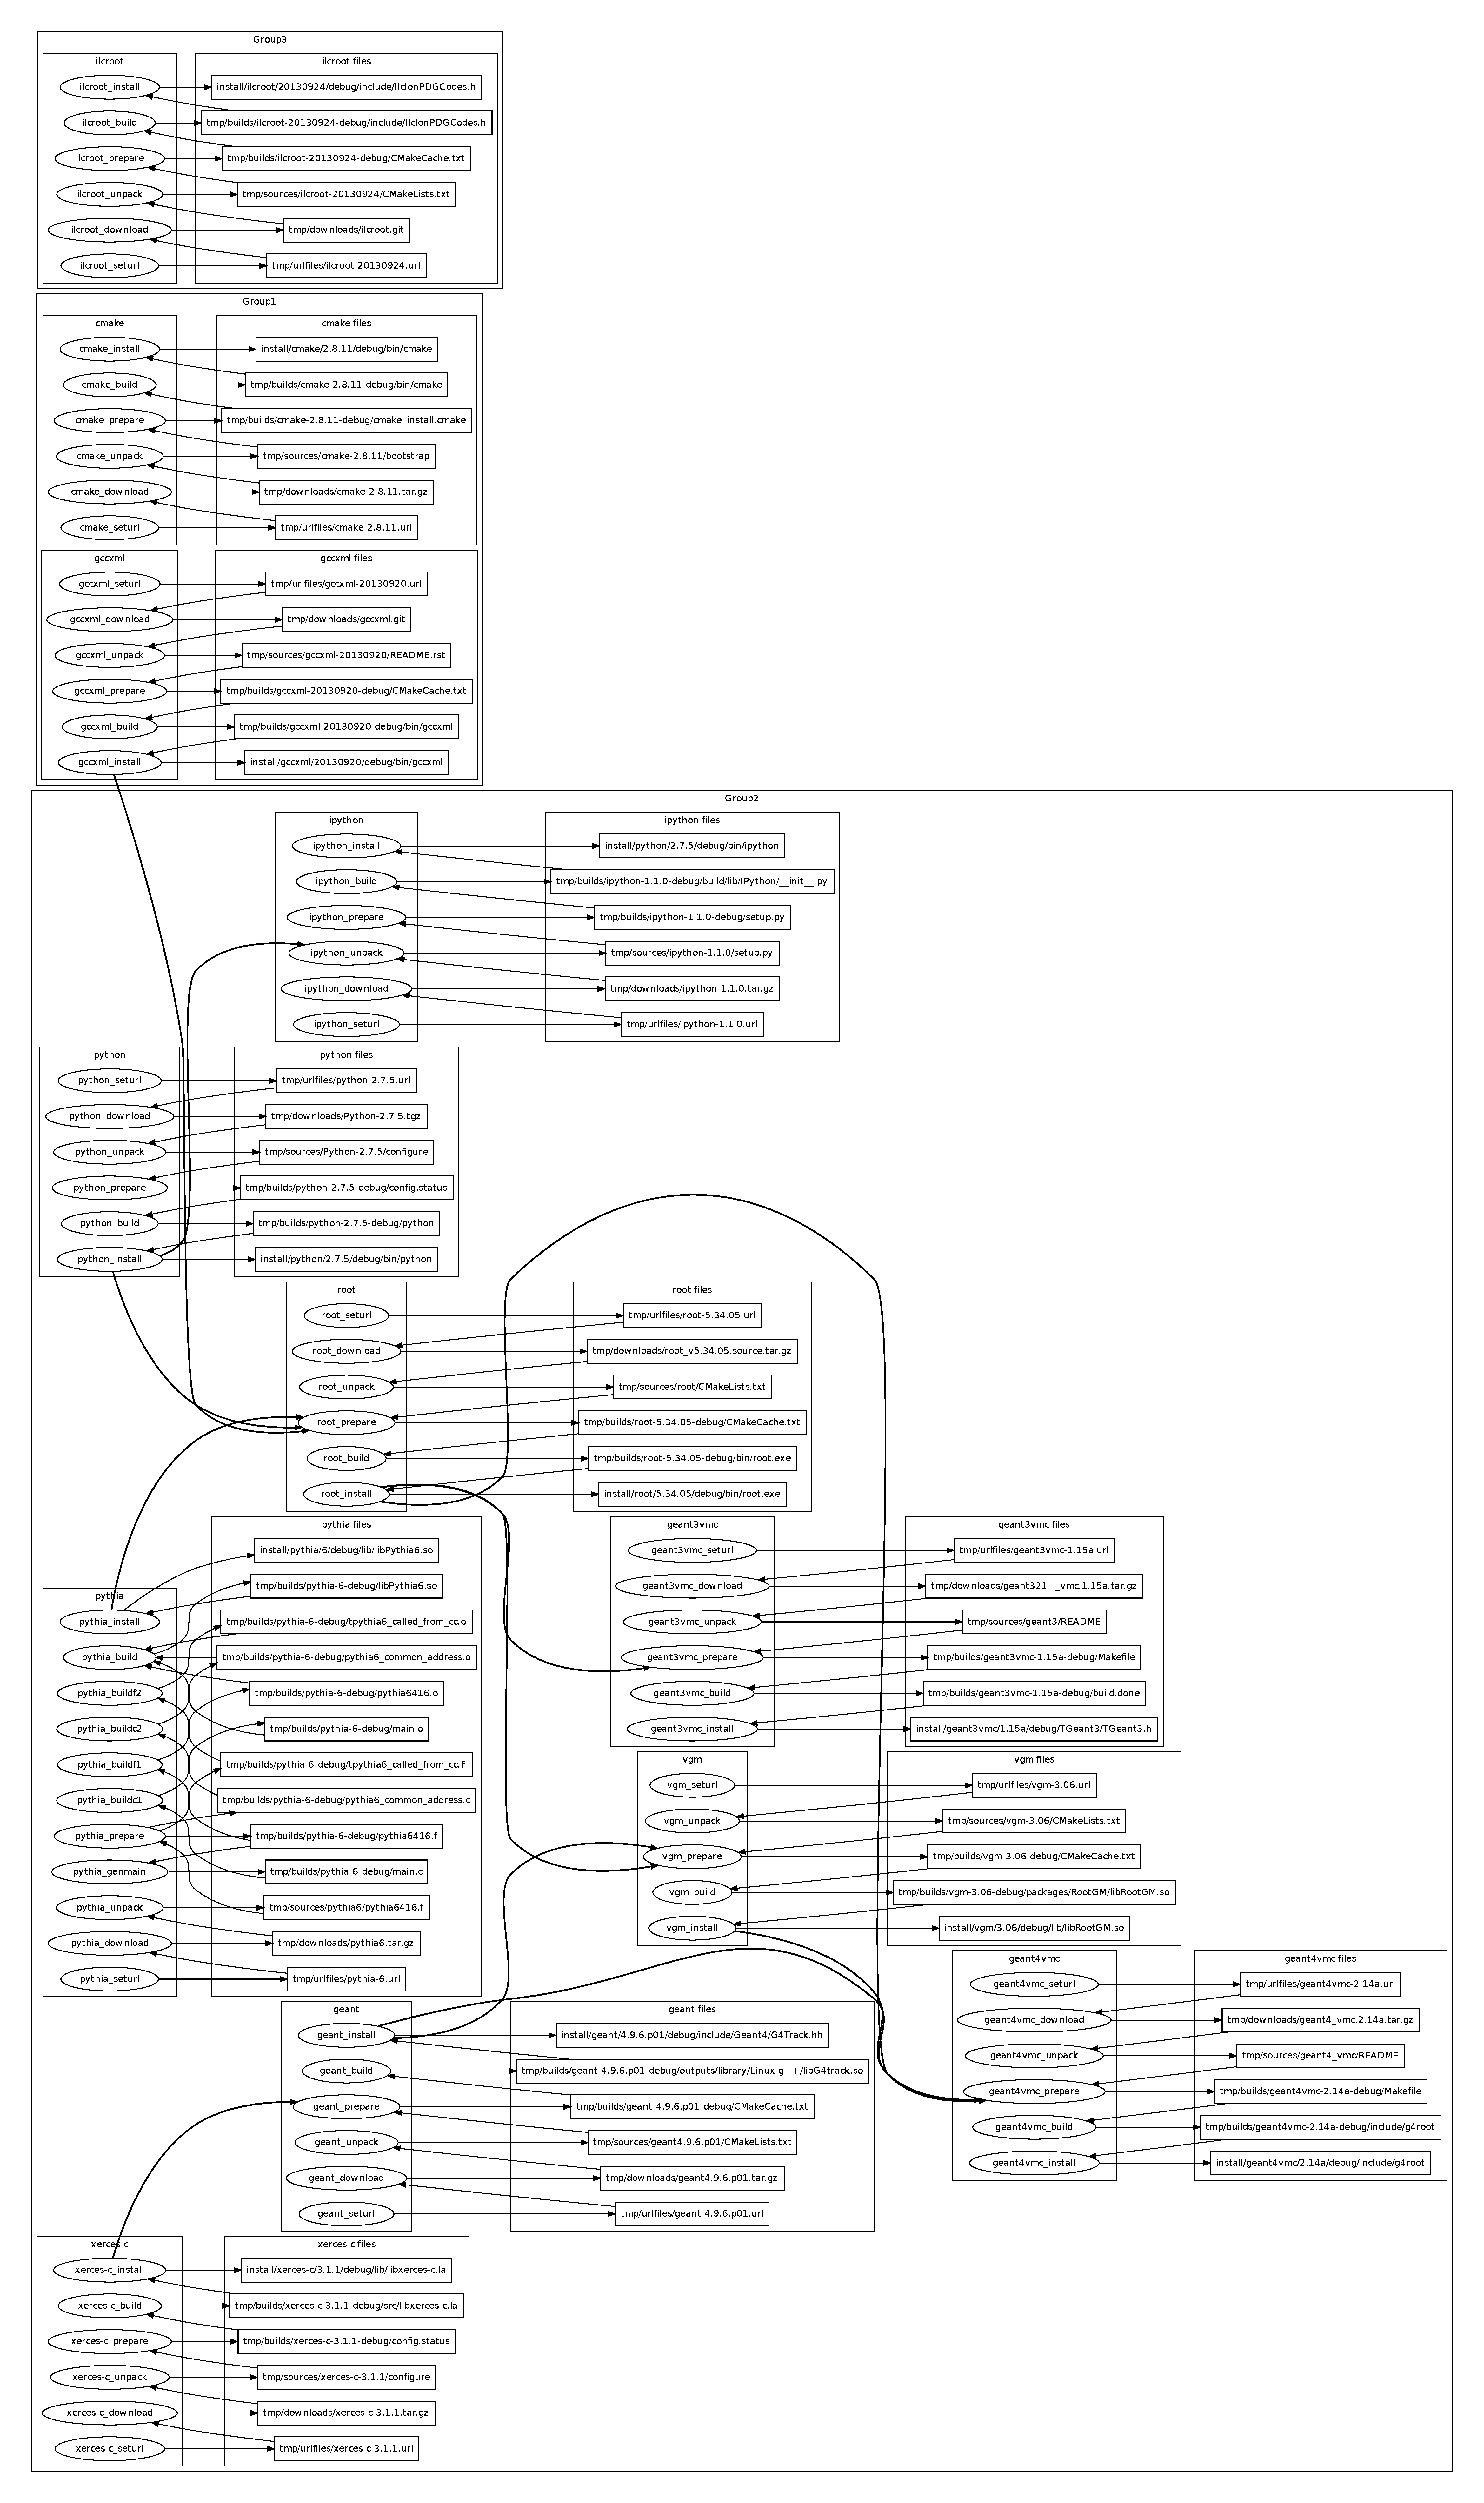
\includegraphics[height=\textheight]{orka}      
    \end{column}
  \end{columns}
\end{frame}

\begin{frame}
  \frametitle{Installation Mechanism}
  
  New installation method: \worch

  \begin{center}
    \url{https://github.com/brettviren/worch} 
  \end{center}

  \begin{itemize}
  \item Previously used a hackish set of shell scripts (\href{https://github.com/brettviren/grinst}{grinst})
    \begin{itemize}
    \item In principle may still work but no longer well supported.
    \end{itemize}
  \item \worch leverages work done for LBNE
  \item supports parallel building and multiple installations
  \end{itemize}

    Status:
    \begin{itemize}
    \item Builds and installs ILCRoot + dependencies
    \item Debug vs. optimized builds not yet fully supported.
    \item User environment management system in development.
      \begin{itemize}
      \item So far supports UPS or Environment Modules
      \item Either way, simple ``\texttt{source ilcroot.sh}'' will be provided
      \end{itemize}
    \item Need to work out comfortable ILCRoot developer environment
      in context of a \worch installation.
    \end{itemize}

\end{frame}

\begin{frame}[fragile]
  \frametitle{How to install with \worch{} -- the easy way}

A couple things to download and a few commands to run:

{\footnotesize
\begin{verbatim}
$ git clone https://github.com/brettviren/worch.git
$ wget https://waf.googlecode.com/files/waf-1.7.13
$ chmod +x waf-1.7.13
$ alias waf=`pwd`/waf-1.7.13

$ cd worch
$ waf --prefix=/path/to/install \
      --orch-config=examples/orka/suite-ilcroot.cfg \
        configure build
...
'build' finished successfully (31m22.537s)
\end{verbatim}
}

  Think of \worch as a ``meta-\app{cmake}'' and \waf like a
  ``meta-\app{make}'' and the \texttt{*.cfg} files like
  ``meta-\texttt{CMakeLists.txt}'' files.

\end{frame}

\begin{frame}[fragile]
  \frametitle{How to install with \worch{} bundles -- the even easier way}

  Bundle everything in one per-release file.

{\scriptsize
\begin{verbatim}
$ wget http://somerver.gov/path/to/<bundle-name-version>
$ chmod +x <bundle-name-version>
$ alias waf=`pwd`/<bundle-name-version>

$ waf --prefix=/path/to/install \
      --orch-config=examples/orka/suite-ilcroot.cfg \
        configure build
...
'build' finished successfully (31m22.537s)
\end{verbatim}
}

Example bundle tested on SL6 and Debian (sid):
\scalebox{0.63}{
  \url{http://www.phy.bnl.gov/~bviren/orka/ilcroot/bundles/worch-ilcroot-builder-20131006}}

Besides simplifying installation, bundles provide one possible method of release management.

\end{frame}

\begin{frame}[fragile]
  \frametitle{Making bundles is easy}

  \begin{center}
    bundle = \waf + \worch + configuration files    
  \end{center}

{
  \small
\begin{verbatim}
$ git clone https://github.com/brettviren/worch.git
$ cd worch/
$ emacs path/to/suite.cfg  # edit config file(s)
$ ./scripts/worch-prepare-bundle <name> path/to/suite.cfg .
$ cp <name> ~/public_html/<public-file-name>
\end{verbatim}
}

Eg:

\begin{verbatim}
./scripts/worch-prepare-bundle \
         worch-ilcroot-builder-20131006 \
         examples/orka .
\end{verbatim}

Bundling is a fairly new idea in \worch and details are subject to change.

\end{frame}

\begin{frame}[fragile]
  \frametitle{Installation on RACF}

  Currently and todo:

  \begin{itemize}
  \item Been poaching from Daya Bay (daya0010) to get SL6
    \begin{itemize}
    \item Avoid SL5, soon to be obsolete, supporting ancient Python hampers \verb|worch| development.
    \item All RACF move to SL6 in October, then can poach off of LBNE too.
    \item Above example can be found in: \verb|daya0010:/data3/bv/orka|
    \end{itemize}
  \item Build exists, need user environment setup
    \begin{itemize}
    \item Anyone can go in and hack their environment by hand right
      now, but it would be tedious.
    \end{itemize}
  \item Identify which other platforms will be used and port to them.
  \end{itemize}
\end{frame}


\begin{frame}
  \frametitle{Summary of ORKA ILCRoot migration and installation}
  \begin{itemize}
  \item Migration to Redmine and \git is done.
    \begin{itemize}
    \item please, no more commits to the old SVN
    \end{itemize}
  \item New, simpler build system in place and ready for testing by others.
    \begin{itemize}
    \item Builds ILCRoot + dependencies on Sci. Linux 6 and Debian (sid)
    \end{itemize}
  \item User and developer environment setup in progress
  \item Will add this info to the Redmine wiki.
  \end{itemize}
\end{frame}

\end{document}


